
\documentclass [french]{sig-alternate-05-2015}
\usepackage{color}
\usepackage[francais]{babel}
\usepackage[utf8]{inputenc}
\usepackage{lmodern}
\usepackage[noend]{algpseudocode}
\usepackage{subcaption}
\usepackage{subfig} 
\usepackage{graphicx}
\usepackage[rflt]{floatflt}
\usepackage{mathrsfs}
\usepackage{multirow}
\usepackage{array}
\usepackage[rflt]{floatflt}
\usepackage{makecell}
\usepackage{usual}
\renewcommand\theadalign{cb}
\renewcommand\theadfont{\bfseries}
\renewcommand\theadgape{\Gape[3pt]}
\renewcommand\cellgape{\Gape[3pt]}

\begin{document}
 

\title{Un modèle pour prendre en compte les relations interpersonnelles dans les stratégies de dialogue}


\numberofauthors{3} 
\author{
\alignauthor Lydia Ould Ouali\\
       \affaddr{LIMSI}\\
       \affaddr{rue John von Neumann}\\
       \affaddr{91405 Orsay }\\
       \email{ouldouali@limsi.fr}
% 5th. author
\alignauthor Nicolas Sabouret\\
       \affaddr{LIMSI}\\
       \affaddr{rue John von Neumann}\\
       \affaddr{91405 Orsay }\\
       \email{sabouret@limsi.fr}
        \and
% 6th. author
\alignauthor Charles Rich\\
       \affaddr{WPI}\\
       \affaddr{Worcester Polytechnic Institute}\\
       \affaddr{Worcester, MA, USA}\\
       \email{rich@wpi.com}    
}


\maketitle
\begin{abstract}
\par Dans cet article, nous proposons un modèle pour un système de dialogue social dans un contexte de négociation coopérative. Le modèle est basé sur 1) des arbres de dialogues, 2) la représentation des états mentaux des interlocuteurs et 3) la prise en compte de la relation sociale pour le choix du prochain acte de dialogue. Nous présentons notre méthodologie de conception de dialogue et l'implémentation de notre système sur un cas pratique de choix coopératif de restaurant.
% But/contribution générale (sans redire le titre...)
% Principaux éléments constitutifs
% Principaux résultats
\end{abstract}


\keywords{Dialogue Social; Relation Interpersonnelle; Négociation Coopérative}

\section{Introduction}


%La modélisation d'agents conversationnels connaît un véritable essor dans différents domaines applicatifs où l'agent est muni d'un système de dialogue lui permettant de jouer différents rôles tels que  le rôle de compagnon \cite{sidner2013always} ou encore de conseiller \cite{bickmore2005s}. 
Les agents conversationnels animés (ACA) sont utilisés dans de nombreuses applications de l'assistance utilisateur \cite{sidner2013always} au compagnon artificiel \cite{sidner2013always, riviere2014aca} en passant par le patient virtuel \cite{annesysteme} ou le recruteur virtuel \cite{jones2012affective}. Tous ces ACA sont munis d'un système de dialogue, plus ou moins élaboré, leur permettant de déterminer quelle phrase choisir en fonction de la situation observée.

Les systèmes de dialogues existants peuvent être divisés en deux catégories: les systèmes orienté tâches et les systèmes de dialogue sociaux. Les systèmes de dialogues orienté tâches sont apparus en premier: ces dialogues se centrent exclusivement sur la collaboration avec l'utilisateur pour satisfaire des tâches communes \cite{allen1995spoken, allen1996robust}. Cependant, un certain nombre de recherches ont montré que l'aspect social ne peut être ignoré dans un dialogue, car ce dernier est social par définition \cite{markopoulos2005case}. Par ailleurs, \cite{moon1998intimate} a démontré que les utilisateurs préféraient interagir avec des agents dotés d'aptitudes sociales, ce qui leur permet de construire une relation sur le long-terme avec l'utilisateur, comme  dans \cite{bickmore2005establishing}. Par conséquent, les chercheurs s'intéressent de plus en plus aux systèmes de dialogues sociaux qui prennent en compte, en plus des tâches à satisfaire, l'aspect social de la conversation dans la mise en œuvre de systèmes de dialogues. Néanmoins, il existe encore peu de recherches qui s'intéressent a la manière dont la relation sociale influence la stratégie de dialogue avec un agent conversationnel. Or, dans le cadre d'une interaction  sociale (voir section \ref{RW}), une modélisation explicite du comportement social de l'agent doit être considérée, car cette dernière influence le dialogue directement, en terme de contenu et de stratégies mises en place par l'agent pour satisfaire ses buts \cite{bickmore2012empirical}. Cependant, deux observations peuvent être faites.

\par Premièrement, la modélisation des comportements sociaux a été largement étudiée en psychologie sociale \cite{dunbar2005perceptions, moon1998intimate}. Plusieurs travaux ont analysés les différentes dimensions qui peuvent affecter le comportement social dans le cadre d'une interaction humain/ humains. Ces notions peuvent être adaptées et utilisées pour le cas d'une interaction humain agent.

 \par Deuxièmement, le dialogue social est défini pas \emph{Laver}\cite{laver1981linguistic} comme un processus d'échange de préférences et d'opinions sur un sujet de conversation. Cet échange de préférences peut conduire les interlocuteurs à mener une négociation - sur leurs préférences - afin de trouver un compromis qui arrangerait les deux participants(e.g deux interlocuteurs qui cherchent un restaurant où dîner). Ce type de négociation est nommé \emph{négociation coopérative}. Nous pouvons donc considérer un dialogue social comme un processus de négociation coopérative sur les préférences dans lequel les stratégies employées par les interlocuteurs pour présenter leurs préférences sont directement affectées par leurs perceptions de la relation interpersonnelle.

\par Dans cette optique, nous proposons dans cet article d'étudier l'impact des relations interpersonnelles sur les stratégies de dialogue employées par interlocuteurs spécialement dans le cadre d'une négociation coopérative. L'article sera structuré comme suit. La section \ref{RW} reprend les travaux récents autour de notre thématique. La section \ref{contribution} sera dédiée à la présentation de notre modèle dialogique préliminaire ainsi que son implémentation. Les perspectives et futurs travaux, plus spécialement l'évaluation du système, seront discutés dans la section \ref{conc}.

\section{Travaux connexes}
\label{RW}
  
La conception d'un système de dialogue social consiste à définir un modèle de conversation où les buts interpersonnels sont mis en avant et les buts orienté tâches, s'ils existent, sont mis en arrière plan \cite{bickmore2005establishing}. Dans le cadre d'une négociation coopérative dans un dialogue social, le but social influence la négociation et la stratégie utilisée. Il existe déjà dans la littérature des travaux sur la négociation coopérative dans le dialogue. Par exemple \cite{Amgoud2002, daskalopulu1998handling} qui ont mis en œuvre des modèles formels de dialogue où les agents sont capables de négocier et même d'argumenter sur leurs choix de préférences. Cependant, ces travaux négligent l'aspect social du dialogue dans la conception des stratégies de négociation. En outre, il a été prouvé que les relations sociales affectent directement le comportement des interlocuteurs \cite{bickmore2012empirical, bickmore2005establishing, moon1998intimate, nass2000does} et par conséquent leurs stratégies dans le dialogue. Par exemple, une personne dominante exprime plus facilement ses préférences et argumente, contrairement a une personne soumise. 

\subsection{ACA sociaux}

\par Il existe dans la littérature des  ACA sociaux  qui arrivent à modéliser leurs relations avec l'utilisateur et la gérer afin d'adapter leur comportements dans la conversation. Le robot \textit{Autom} \cite{kidd2005sociable}, qui est placé dans les maisons des utilisateurs pour une intervention sur le long terme, s'intéresse principalement à trois facteurs de relations avec l'utilisateur: \textit{l'engagement}, \textit{la confiance} et \textit{la motivation}. Il construit cette relation sur trois étapes: la prise de connaissance, la construction des relations et enfin la maintenance de la relation. Le système dispose d'un nombre limité d'actes de langage pour  entretenir sa relation avec l'utilisateur. Dans notre modèle, nous utiliserons aussi des actes de dialogue pour communiquer avec l'utilisateur.

\textit{FitTrack} \cite{bickmore2005s} utilise un large éventail de techniques tirées de la psychologie sociale des relations pour accroître le lien social avec l'utilisateur au cours de l'intervention. Cependant, les comportements sociaux ne sont pas généré dynamiquement. Ils sont préalablement codé dans le dialogue de l'agent qui est basé sur une machine d'états fini et apparaissent selon un calendrier pré-défini. Ainsi, le modèle relationnel évolue implicitement dans le temps. Au contraire, dans nos travaux, nous voulons que le dialogue s'adapte dynamiquement à l'évolution de la relation interpersonnelle.

\textit{REA} \cite{bickmore2005establishing} est un agent incarné grandeur nature qui joue le rôle d'un agent immobilier. Le planificateur décide dynamiquement de choisir entre le dialogue social ou sur des un dialogue orienté tâches. Un des facteurs de choix de dialogue est basé sur une évaluation de la relation actuelle avec l'utilisateur. La relation a été modélisé en utilisant un modèle tridimensionnel \cite{svennevig2000getting} et une dimension de \textit{confiance} a été ajoutée au système pour améliore les performances. La mise à jour des relations est basée sur le nombre et le contenu des mouvements de conversation. Cependant, dans REA, la partie "sociale" du dialogue est séparée de la tâche: l'agent utilise les dialogues sociaux pour "briser la glace" avec l'utilisateur lorsqu'il pense que c'est nécessaire. Au contraire, notre proposition est d'intégrer \textit{au sein du dialogue de tâche} la prise en compte de la dimension sociale dans le choix des énoncés et dans la prise de décision de l'agent.

\textit{AlwaysOn} \cite{sidner2013always} est un agent incarné pour une interaction avec les personnes âgées sur un long terme. Ce système s'intéresse à l'étude de l'engagement et des relations qui se créent avec l'utilisateur au cours des interactions. En effet, il dispose d'un planificateur qui décide quelle activité suggérer à l'utilisateur en fonction de l'évolution de la relation de \textit{proximité}. L'interaction se fait via un dialogue textuel et l'utilisateur choisit sa réponse à partir d'un menu. Dans notre modèle, nous souhaitons permettre à l'utilisateur de formuler n'importe quelle proposition (dans le vocabulaire défini à l'aide des actes de dialogues) avec ses préférences, ce qui ne peut pas être géré avec un menu limité de valeurs.

Notre travail s'inscrit donc dans la continuité de ces travaux sur les dialogues sociaux. Nous modélisons un agent conversationnel qui pourra percevoir sa relation avec l'utilisateur et adapter ses stratégies de négociation et dialogue.

\subsection{Formalisme des relations interpersonnelles}
\label{RI}
Il existe de nombreuses représentations des relations interpersonnelles dans la littérature. Cependant, la représentation dimensionnelle demeure la plus courante. Elle consiste à projeter les relations dans un cercle de dimensions \cite{wiggins1985interpersonal}. Par conséquent, toute relation peut être située et évaluée dans cet espace dimensionnel \textit{continu}. Un des modèles les plus connus est celui de Svennevig \cite{svennevig2000getting} qui divise les relations interpersonnelles sur quatre dimensions: dominance, familiarité, affect et solidarité. Nous nous intéressons plus particulièrement à la relation de dominance, qui est un comportement social typique qu'on peut observer dans les interactions humaines \cite{dunbar2005perceptions}. On retrouve différentes définitions de la relation de dominance dans la littérature mais elles convergent toutes à définir la dominance comme le pouvoir d'influencer le comportement d'autrui afin d'asseoir son autorité\cite{dunbar2005perceptions,rogers1979domineeringness,moon1998intimate}.

La position de dominance en terme de relation interpersonnelle peut être manifeste \cite{dunbar2005perceptions} lorsque l'assertion de dominance manifestée chez un interlocuteur rencontre forcement  l'acquiescement de l'autre \cite{rogers1979domineeringness}. Elle peut aussi être latente \cite{komter1989hidden} lorsque l'interlocuteur dominant n'a pas conscience de sa position de dominance. Ce genre de comportements peut affecter l'interaction de manière positive ou négative. L'apport positif consiste a permettre par exemple d'entretenir la conversation, d'orienter la tâche courante de l'interaction, de prendre des décisions rapides et efficaces et de définir des conclusions. Cependant, ce même comportement peut affecter l'interaction de façon négative: la personne dominante peut étouffer l'autre et ne pas lui laisser la possibilité d'exprimer ses opinions. Cette expression verbale de la dominance peut être perçue comme offensive et injustifié par l'autre et peut mener a des conflits dans le dialogue si les deux interlocuteurs sont dans une position de dominance avec des opinions différentes \cite{zablotskaya2012relating}.

\par Plusieurs approches existent pour détecter les comportements de dominance dans l'interaction. Ces indicateurs peuvent être soit verbaux ou non verbaux. Les indicateurs non verbaux peuvent être vu dans les expressions faciales tels que le ratio de dominance visuel \cite{dunbar2005perceptions}. Le contrôle de la posture et les gestes sont aussi perçue comme une comportement dominant: \cite{hall2005nonverbal} ont ainsi montré que les personnes dominantes avaient tendance à plus utiliser les gestes tels qu'une poignée de main ou bien une plus grande fréquence "invasive touch". Les indicateurs verbaux incluent: la fréquence d'intervention dans l'interaction, leurs durée (comme dans  \cite{dunbar2005perceptions}), l’expression des opinions
et la critique, les suggestions, les demandes, les réactions, les aveux d'ignorance (comme dans \cite{zablotskaya2012relating}), les interruptions ou les
changements de conversation.

Notre objectif est donc de reproduire ces comportements liés à la relation de dominance dans un agents conversationnel animé. Dans cet article, nous nous limitons aux comportements verbaux et plus précisément éléments en rapport avec la gestion du dialogue.

\section{Contributions}
\label{contribution}

\par Afin de définir un système de dialogue social dans lequel la relation de dominance régit le choix du prochain énoncé, nous avons d'abord enregistré des dialogues entre deux personnes afin d'observer leurs comportements dans un cadre de dialogue social de type "négociation coopérative". Nous avons annotés et analysé les dialogues. Cette étude nous a livré un ensemble de comportements  que nous avons ensuite reproduit dans des jeux de dialogues dans le modèle D4G utilisé au sein de la plate-forme de dialogue Disco \cite{rich2009building}. 
 Les informations collectées grâce l'observation des comportements humains nous a guidés dans la conception de notre modèle dialogique qui comprend un modèle mental de l'environnement de l'agent et un modèle lui permettant de mener une négociation coopérative. 
En parallèle, nous avons défini un module de communication comportant cinq actes dialogiques correspondant aux différents types d'échanges observés pendant la négociation. Nous présentons dans cette partie notre démarche de conception, notre proposition de modèle de dialogue ainsi qu'une première implémentation.

\subsection{Analyse de la structure du dialogue}

Pour mieux comprendre les comportements liés à la dominance qui peuvent apparaître durant une négociation coopérative, nous avons enregistré deux dialogues dans lesquels les interlocuteurs avaient pour but de trouver un restaurant où dîner sur Paris. Les dialogues enregistrés ont ensuite étaient annoté et analysé en se basant sur les travaux de Sidner \& Grosz \cite{grosz1986attention}. Nous avons effectué une analyse de \textit{la structure linguistique}  en décomposant le dialogue en segments de dialogue (DS). Cette segmentation du dialogue en DS nous a permis d'extraire un squelette de dialogue pour la tâche "choix d'un restaurant" et d'identifier les critères de la négociation dans ce domaine: le type de cuisine, l'ambiance, le prix et l'emplacement. Cela nous a aussi permis de définir un ensemble d'actes de dialogues pour notre agent, obtenus à partir des principaux actes de langages récurrents observés dans ces enregistrements.

Nous avons aussi pu vérifier les propositions de la littérature concernant l'impact de la dominance sur la stratégie de dialogue. Premièrement, l'interlocuteur dominant a effectivement tendance à influencer le dialogue, c'est-à-dire à initier de nouveaux DS. Deuxièmement, il prend la parole plus souvent et exprime explicitement ses opinions: cela se traduit par un nombre plus élevé d'actes de dialogue dans un même DS. Enfin, les interlocuteurs soumis ou neutres défendent leurs préférences moins âprement, c'est-à-dire qu'ils utilisent des tournures moins explicites pour exprimer leurs refus. Dans notre modèle, nous avons choisi pour l'instant de ne pas représenter le style linguistique et la partie argumentative dans le dialogue (\emph{c.-à-d.} la justification des choix) et de nous limiter aux actes de dialogue. Pour reproduire ce phénomène dans notre système, nous avons donc utilisé des actes de dialogues détournés comme répondre à une proposition par une expression de préférence ("ah, le chinois, je n'aime pas trop") plutôt qu'un refus ("non, pas le chinois").

\subsection{Modèle formel du dialogue}
\par Le modèle proposé vise à concevoir un agent conversationnel capable de mener une négociation coopérative sur un sujet de conversation sociale et d'adapter ses stratégies de dialogue en fonction de sa perception de la relation interpersonnelle avec l'utilisateur. Le modèle proposée (illustré dans
 la \fig{modele}) se compose de trois principaux modules: un \textit{état mental} regroupant les préférences de l'agent et celles de l'utilisateur, un \textit{module de communication} comprenant les actes de langage que l'agent utilise pour dialoguer et enfin un module qui sauvegarde le \textit{contexte du dialogue} à savoir l'historique des informations échangées durant le dialogue (en termes de préférences et propositions échangées).
\begin{figure}
	\centerline{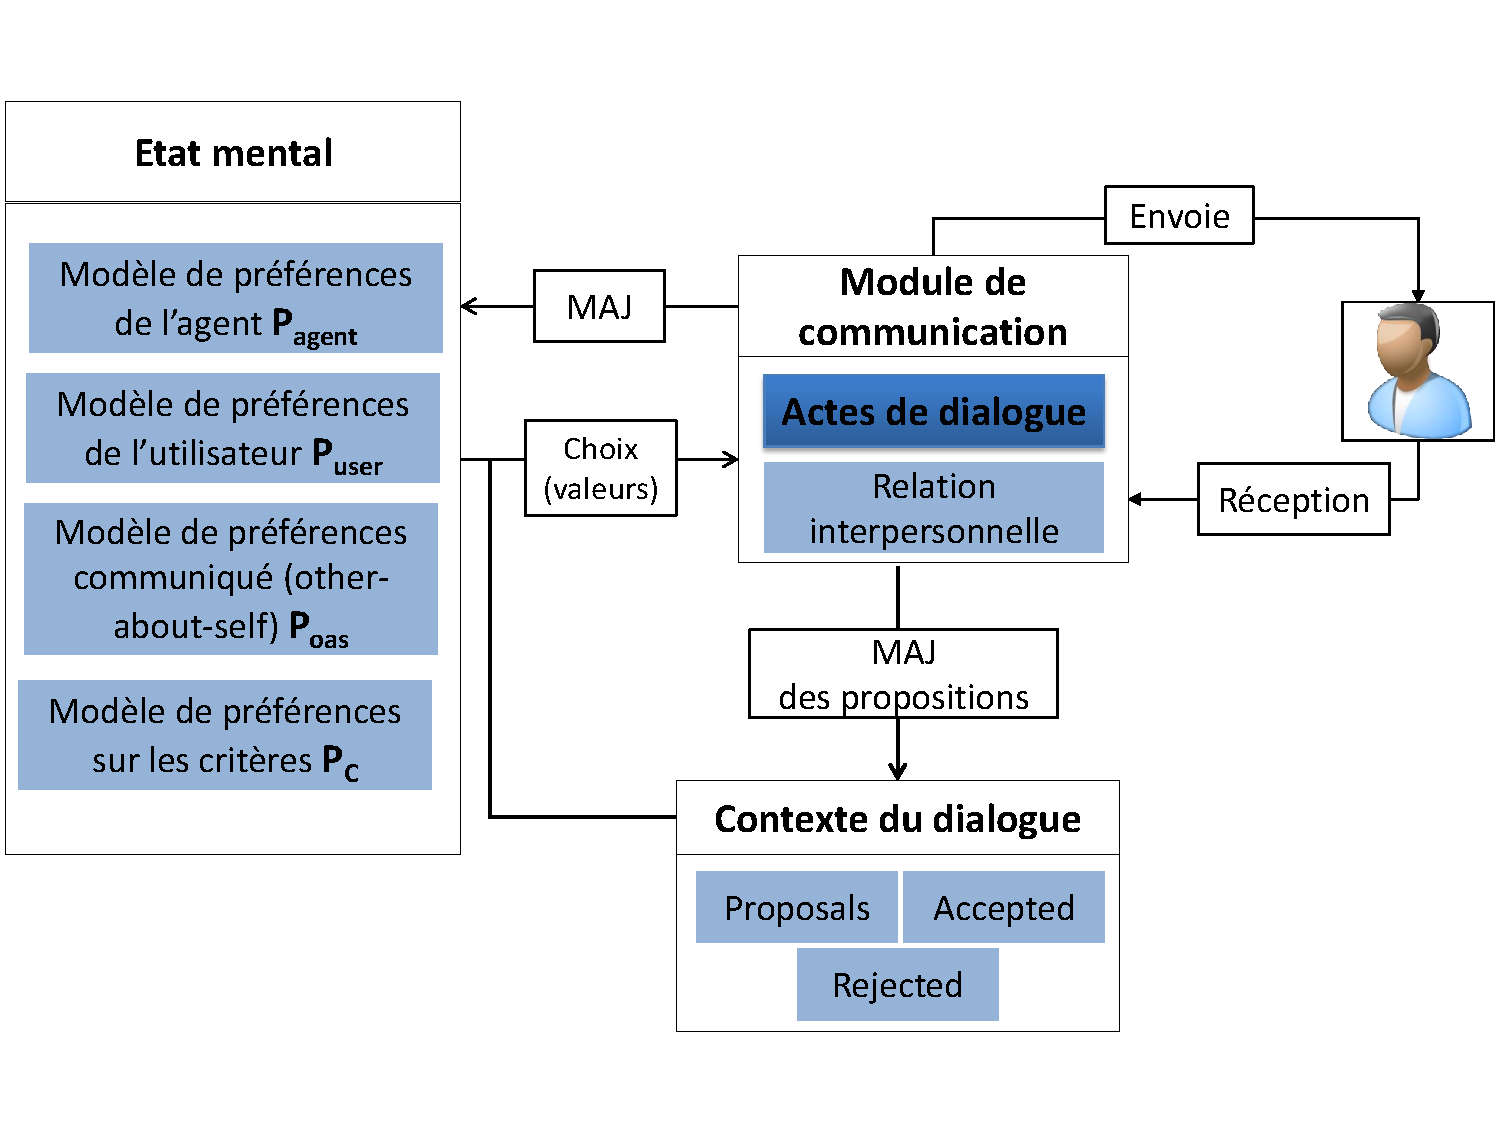
\includegraphics [width=3.25in]{figs/modele_v1.pdf}}
	\defig{modele}{Architecture du modèle de dialogue.}
\end{figure}

\subsubsection{L'état mental}

Mener une négociation coopérative sur un sujet défini implique un processus décisionnel de la part des interlocuteurs régi par les préférences de chacun \cite{laver1981linguistic}. C'est pourquoi nous définissons les éléments suivants.

\paragraph{Le domaine de connaissances}
Nous considérons un ensemble d'options $\mathcal{O}$ dans le domaine de négociation (par exemple, un ensemble de restaurants pour une négociation sur le choix de restaurants). L'objectif de la négociation coopérative est de choisir ensemble un élément de l'ensemble $\mathcal{O}$. Nous considérons de plus un ensemble de critères $\mathcal{C}$ qui reflètent leurs caractéristiques (par exemple, pour les restaurants, la cuisine, le prix, l'ambiance et l'emplacement). Pour chaque $o\in\mathcal{O}$ et pour chaque $c\in\mathcal{C}$, nous notons $v(o,c)$ la valeur attribuée à $o$ pour le critère $c$ (par exemple, Ginza est un restaurant japonais coûteux : $v(prix, Ginza) = couteux $ et $ v (cuisine, Ginza) = japonais$). Nous notons $\mathcal{D}_c$ le domaine de valeur du critère $c$.

\paragraph{Notion de préférence}
L'agent est capable d'exprimer ses préférences sur le domaine de connaissance. Nous définissons une préférence $P$ comme une relation \emph{transitive} et \emph{antisymétrique} définit sur un ensemble d'éléments \emph{A}, tel que pour $(a,b) \in \emph{A}^2$, $P(a,b)$ représente le fait que $b$  est préféré à $a$. $P$ définit donc un ordre \emph{partiel}.

Chaque agent dispose d'un ensemble de préférences sur les critères, notés $P_c$. Par exemple $P_{cuisine} (Italien, Japonais)$ signifie que l'agent préfère la cuisine japonaise à l'italienne. Nous définissons des éléments maximaux et minimaux pour la notion de préférences à l'aide de la notation:
\begin{itemize}
	\item  \emph{P(*,a)}  = \{$\forall$ \emph{x}$\in$\emph{A}, \emph{P(a,x)}\}, représente le fait que  \emph{a} est l'élément  \textit{le plus préféré} dans \emph{A}.
	\item Par opposition, \emph{P(b,*)} = \{$\forall$ \emph{x}$\in$\emph{A}, \emph{P(x,b)}\} signifie que \emph{b} est l'élément \textit{le moins préféré} dans l'ensemble \emph{A}. 
\end{itemize}

\paragraph{Ensembles de préférences}
Nous définissons alors une base de préférences de l'agent et de l'utilisateur qui comprend trois éléments:
\begin{itemize}
	\item Un ensemble $Pc$ de préférence sur les critères $C$ qui définit l'importance de chaque critère \emph{pour l'agent} dans la prise de décision.
	\item Un ensemble $\mathcal{P}_{self}$ qui représente l'ensemble des $P_c$ de l'agent pour chaque critère $c$: c'est le modèle de préférences \emph{de l'agent}.
	\item Un ensemble $\mathcal{P}_{other}$ qui représente le modèle de préférences \emph{de l'utilisateur} sur la base de ce que l'agent aura acquis au cours du dialogue.
\end{itemize}

De plus, l'agent conserve les préférences qu'il communique à l'utilisateur durant la négociation qu'on note $\mathcal{P}_{oas}$ (\textit{other about self}). En effet, il est important pour l'agent de savoir ce qu'il a déjà communiqué pour évaluer la relation de dominance avec l'utilisateur, en s'appuyant sur un petit module de la théorie d'esprit à base de règles simples comme, par exemple, ``si l'interlocuteur contredit une préférence que j'ai déjà énoncé, c'est qu'il est plutôt dominant''.

% \par Dans ce qui suit, nous présenterons le modèle formel de préférences utilisé pour la représentation de l'état mental de l'agent.


%
%\par Notre but est de définir des préférences sur les options de la négociation.  Nous retrouvons dans la littérature plusieurs méthodes de calcul des préférences d'une option \cite{dodgson2009multi}. Ces méthodes nommées décision multi-critères calculent les préférences d'une option selon les performances de cette dernière sur l'ensemble des critères qui la définissent. Dans l'ensemble\cite{dodgson2009multi}, le calcul des préférences d'une option est fait par inférence à partir des préférences enregistrées sur les valeurs de ses critères. Cette inférence peut être réalisée grâce à différentes méthodes comme la fonction de somme pondérée \cite{yager2012ordered} ou encore les intégrales de Choquet \cite{chouquet1953}. \\
%

\subsubsection{Processus décisionnel basé sur les préférences}
Afin de trouver une option qui satisfasse les préférences des deux interlocuteurs, l'agent doit être en mesure de calculer ses préférences sur les différentes options dans $\mathcal{O}$. La relation de préférence entre deux options est calculée à partir des préférences de l'agent grâce a une fonction de décision multi-critères. Nous avons sélectionné pour notre modèle une fonction de somme pondérée par le rang de chaque critère \cite{yager2012ordered}.

Pour toute relation de préférence $P$ et pour tout élément $a\in A$, nous définissons $score_A(a)$ le nombre de successeurs de $a$ dans $P$ (définis par transitivité de $P$). Nous définissons ensuite le rang $rang_A(a)$ à partir du score de tous les $a_i\in A$ et en les triant par score croissant.

Soit $o\in \mathcal{O}$ une option. L'utilité de l'option pour l'agent est définie par:

\[U(o) = \sum_{c \in \mathcal{C}}  rang_{\mathcal{C}}(c) \times score_{\mathcal{D}_c}\left( v(o, c) \right) \] 


\par La relation de préférence entre deux options est donc calculée en comparant leurs utilités. 
\[ P(o_1, o_2)  = \left \{
\begin{array}{l}
P(o_1, o_2)$ \textit{si} $U(o_1) < U(o_2) \\
P(o_2, o_1)$ \textit{si} $U(o_1) > U(o_2) 
\end{array}
\right .\]

\subsubsection{Contexte du dialogue}
\par Durant le dialogue, les deux interlocuteurs échangent des informations sur leurs préférences (par exemple "j'aime bien le japonais") et suggèrent des propositions pour le choix d'un critère (par exemple, "allons manger indien") ou sur les options ("allons au restaurant Ginza").

Afin de capturer ces informations, nous définissons une proposition comme un couple $(Type, Valeur)$ où $Type$ est soit un type d'option qui encapsule le (''Restaurant`` dans notre exemple), soit un critère, et $Valeur$ est
\begin{itemize}
	\item 	soit $Type$  est le thème de négociation (”Restaurant“ dans notre exemple)
	et $Valeur$ est une option $O \in \mathcal{O}$;
	\item soit Type est un critère  $c \in \mathcal{C}$?  et et $Valeur$ est valeur de critère $v \in \mathcal{D}_c$."
\end{itemize}
Par exemple, $(Restaurant,Ginza)$ représente la proposition "allons au restaurant Ginza" alors que $(Cuisine,Indien)$ représente la proposition "allons manger indien".

Afin de garder trace de toutes les propositions soumises durant le dialogue, nous définissons:
\begin{itemize}
	\item $ Proposed$ la liste de toutes les propositions ouvertes dans le dialogue.
	\item $ Rejected$ la liste des propositions rejetées.
	\item $ Accepted$ la liste des propositions acceptées. Notons qu'il suffit qu'une seule \emph{option} soit acceptée pour clore la négociation coopérative.
\end{itemize}

\subsubsection{Module de communication}

\paragraph{Actes de dialogue}
\par Dans notre système, l'agent et l'utilisateur communiquent en utilisant des actes de dialogues au sens de Searle \cite{searle1969speech}. Chaque acte de dialogue est muni de préconditions et d'effets qui mettent à jours l'état mental de l'agent à propos des préférences de l'interlocuteur et de l'état des propositions (les ensembles $\mathcal{P}_{self}$ et $P_c$ ne sont jamais modifiés, contrairement à ce qui serait fait en théorie de l'argumentation, par exemple). 

Le tableau \ref{tab: utt} décrit l'ensemble des actes de dialogue que nous avons retenus pour notre modèle de négociation coopérative. À titre d'exemple l'acte de dialogue "State.Preference" permet à l'agent d'exprimer une préférence sur n'importe quel domaine. Ainsi, "je préfère le chinois au japonais" est exprimé par:
 $State.Preference_{cuisine}(\textit{Japanese , Chinese})$.

\begin{table*}	
	\centering
	\begin{tabular} {|m{4cm}|m{2cm}|m{2.5cm}|m{3cm}|m{2.5cm}|}
		
		\hline 
		\thead{Utterance} & \multicolumn{2}{c|} {\thead{Preconditions}  } &  \multicolumn{2}{c|} {\thead{Effects}  } \\
		\hline 
		\makecell{State.Preference(\textit{$a,b$}):\\ ``I prefer $a$ over $b$''}& \multicolumn{2}{c|} {\makecell{ $(a,b)\in$ $\mathcal{P}_{self}$ } }&\makecell{ \textit{(hearer case)} \\ $add((a,b)$, $\mathcal{P}_{other})$ } & \makecell{\textit{(speaker case)} \\ $add((a,b)$, $\mathcal{P}_{oas})$}  \\
		\hline
		\makecell{Ask.Preference(\textit{$a,b$}):\\``Do you prefer $a$ to $b$'' ?}& \multicolumn{2}{c|} {\makecell{ $ (a,b) \notin \mathcal{P}_{other} $} }&
		\multicolumn{2}{c|} {\makecell{None} } \\
		\hline
		\makecell{Propose(\textit{Proposal(T,V)}):\\``Let's choose  \textit{V}''}& \multicolumn{2}{c|} {\makecell{$ Proposal(T,V) \notin  Proposed$} }&\multicolumn{2}{c|} {\makecell{ $add(Proposal(T,V), Proposed)$ }} \\
		\hline
		\makecell{Accept(\textit{Proposal(T,V)}):\\``Okay, let's choose \\ \textit{V} for \textit{T}''}& \multicolumn{2}{c|} {\makecell{$Proposal(T,V) \in Proposed$ \\ $ Proposal(T,V)\notin Accepted$} } & \multicolumn{2}{c|} { \makecell{$add(Proposal(T,V), Accepted)$\\$ remove(Value, Proposed)$}  }  \\
		\hline
		\makecell{Reject(\textit{Proposal(T,V)}):\\`` Sorry, I would choice \\ something else.''}& \multicolumn{2}{c|} { \makecell{$Proposal(T,V) \in Proposed$ \\$Proposal(T,V)\notin Rejected$}  } & \multicolumn{2}{c|} {\makecell{ $add(Proposal(T,V),Rejected)$ \\$remove(Proposal(T,V), Proposed)$}} \\
		\hline
	\end{tabular}
	\caption{\label{tab: utt} Sémantique des actes de dialogue}
\end{table*}

\paragraph{Arbres de dialogue}
La gestion du dialogue se fait à l'aide d'arbres qui décrivent, pour chaque acte de dialogue, l'ensemble des réponses que l'agent peut sélectionner. Par exemple, suite à un acte Propose, l'agent peut répondre par un Accept, un Reject ou un autre Propose ("User: Allons au Chinois. Agent: Et si nous allions plutôt au Japonais?"). En plus des préconditions de chaque acte, ces arbres définissent des conditions sur la relation de dominance pour décider quelle réponse est adoptée. Dans l'exemple précédent, l'agent doit être dominant pour répondre à un Propose par un autre Propose. Ces conditions sont définies d'après les observations de la littérature présentées dans la section\ref{RI}.


\subsection{Implémentation du modèle de dialogue}

\par Nous avons réalisé une première implémentation de notre système de dialogue à l'aide du logiciel Disco \cite{rich2009building} qui gère la création d'actes de dialogue ainsi que la génération d'arbres de dialogue. Nous avons implémenté un modèle générique de l'état mental et nous l'avons instancié sur la tâche de choix d'un restaurant.

\subsubsection{Présentation de Disco}
Disco est une implémentation d'un ``collaborative discourse manager'' inspiré d'une théorie de dialogue collaboratif comme Collagen \cite{rich1997collagen}. Disco est un système qui permet la génération de dialogues orienté tâches pour lequel il utilise le formalisme des HTNs (Hierarchical Task Networks) \cite{erol1994htn} pour la gestion des tâches. Il est implémenté avec le standard ANSI/CEA-2018 : chaque tâche est définit avec des préconditions, des effets et des postconditions. Les tâches sont regroupées par \emph{recettes} munies de conditions d'applicabilité.

De plus, Disco a été étendu avec un module génération d'arbres de dialogues afin de communiquer et collaborer avec l'utilisateur pour la réalisation des tâches. Ce module est nommé Disco for Games (D4g) et permet de définir des sémantiques d'actes de dialogue. D4g est déjà fourni avec un ensemble d'actes de dialogue.

Nous avons complété ce système avec les actes de dialogues présenté dans la section précédente afin qu'il puisse supporter la négociation sur les préférences. Les conditions des actes de dialogue sont exprimées par des préconditions sur les tâches et le choix de l'acte suivant la relation de dominance est implémenté dans les recettes.

\subsubsection{Génération de dialogue} 
 \par Le système de dialogue offre à l'utilisateur la liberté de choisir n'importe quel acte de dialogue pour son tour de parole. Disco déroule alors l'arbre de dialogue correspondant de gauche à droite (en commençant par la branche la plus à gauche). La première branche applicable rencontrée est directement exécutée sans vérifier les branches restantes.
 Par exemple, les réponses que l'agent peut générer quand il reçoit un \emph{StatePreference} de la part de l'utilisateur sont présentées dans la \fig{state}.

 \begin{figure} [h]
 	\centerline{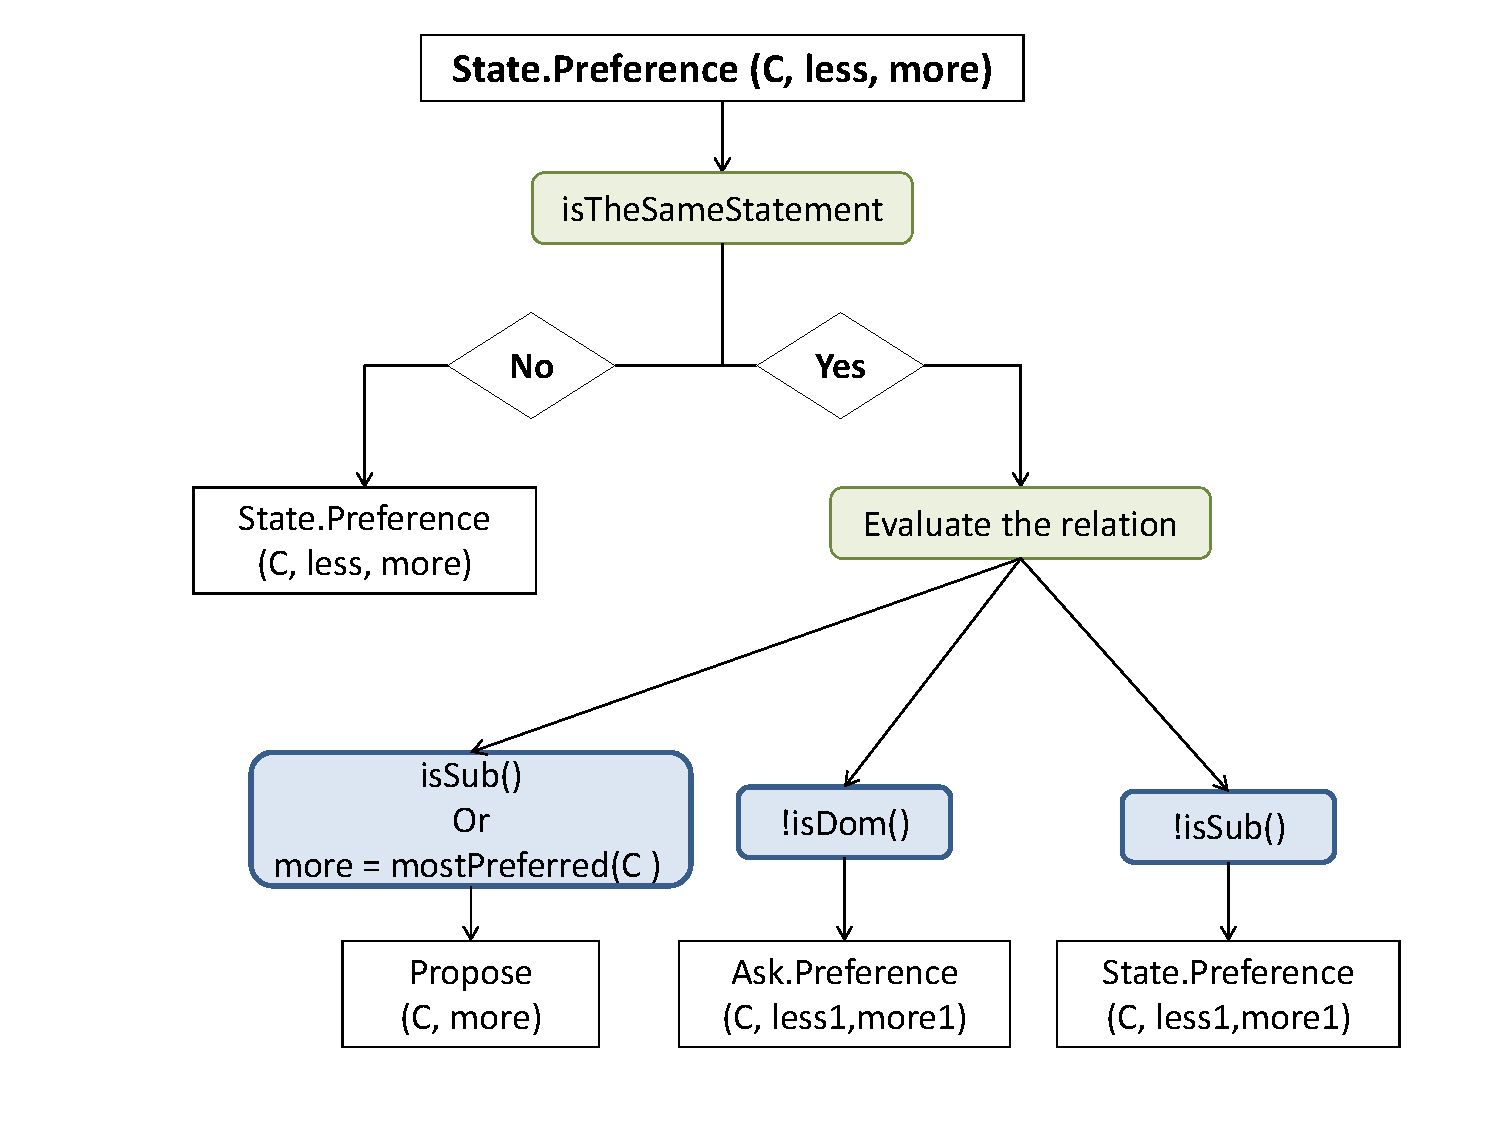
\includegraphics[width=3in]{figs/statePref.pdf}}
	\vskip 8pt
 	\defig{state}{Les réponses générés suite à un StatePreference}
 \end{figure}

Ainsi, dans l'exemple donné, le comportement standard qu'un agent adopte à la réception d'un StatePreference est de donner son opinion sur les valeurs exprimées (c-à-d que l'agent calcule ses préférences sur \textit{less} et \textit{more}). Cependant, si l'agent a déjà exprimé ses préférences sur ces valeurs, il va vouloir choisir un autre acte de dialogue en fonction de la relation sociale:
 \begin{itemize}
 	\item Si l'agent est soumis ou si il a la même préférence que l'utilisateur, il va proposer de choisir la valeur préférée de l'utilisateur
 	\item Sinon, si l'agent est soumis ou neutre, il va vouloir en apprendre d'avantage sur  les préférences de l'utilisateur.
 	\item Enfin, si l'agent est neutre ou dominant, il exprime ses préférences sur d'autre valeurs du critère \emph{C} discuté ou, dans le cas où il a déjà exprimé toutes ses préférences sur les valeurs du critère discuté, sur un autre critère non encore discuté.
 \end{itemize}
 
\paragraph{Exemple de dialogue}
Voici un exemple de dialogue produit par le système. Les réponses de l'utilisateur sont pour l'instant traduites manuellement en commandes \emph{execute} en Disco:
{\small
\begin{verbatim}
Agent says "What type of cuisine do you prefer?"
> execute StatePreference / null / restaurant.Cuisine.FRENCH
User says "I like FRENCH most."

Agent says "I like FRENCH less than CHINESE."
> execute Propose / CreateProposal(restaurant.Cuisine.CHINESE)
User says "Let's choose CHINESE."

Agent says "Okay, let's choose CHINESE."
...
\end{verbatim}
}

\section{Conclusions et perspectives}
\label{conc}
Dans cet article, nous avons présenté un modèle de dialogue qui permet à l'agent de mener une négociation coopérative et d'adapter sa stratégie de négociation en fonction de la relation interpersonnelle construite avec l'utilisateur. Nous avons effectué une première implémentation de ce système. 

\par La prochaine étape de nos travaux se concentrera sur l'évaluation d'un tel système de dialogue social. Tout d'abord, nous souhaitons évaluer si le comportement de l'agent durant le dialogue traduit le comportement attendu. Ce type d'évaluation peut s'effectuer à l'aide de tests perceptifs avec des observateurs externes \cite{bickmore2012empirical}.

\par Ensuite, nous voudrions étudier l'impact de la prise en compte des relations sociales sur la qualité du dialogue: il s'agit alors de vérifier, au cours d'une interaction avec l'agent, non seulement que l'utilisateur perçoit la présence des comportements sociaux de l'agent, mais aussi que ces comportements ont un impact sur l'engagement de l'utilisateur et la qualité de la négociation menée durant le dialogue. L'hypothèse est que l'interaction est plus agréable avec un agent social et que la négociation sera plus rapide à converger.

\par Enfin, au delà de ces perspectives liées à la validation, nous souhaitons étendre notre modèle de relation interpersonnelle (RI). La proposition actuelle considère que la RI est donnée a priori à l'initiation du dialogue et non actualisée lors de l'interaction. Nous souhaitons munir notre système d'un module simple de \emph{théorie de l'esprit} qui lui permettra d'évaluer la dominance de l'utilisateur en fonction de ses choix d'actes de dialogue et de comprendre ses intentions pour mieux cerner son comportement. Nous espérons que cette extension améliore la gestion des stratégies de négociation coopérative de l'agent, qui serait alors capable de s'adapter à l'utilisateur.
 
%=====================================================================================================
\vskip 5pt
\bibliographystyle{abbrv}
\bibliography{Library}

\end{document}
